\begin{figure}[ht!]
    \centering
    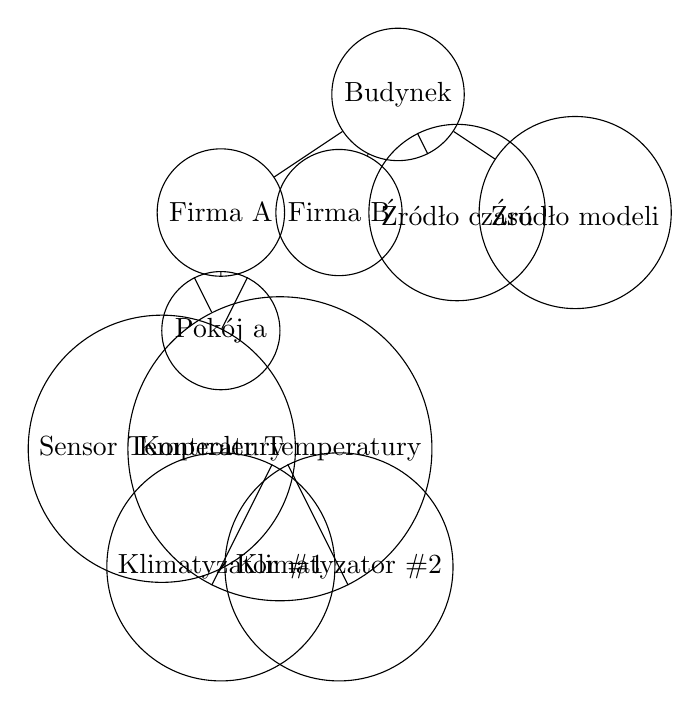
\begin{tikzpicture}[
        interface/.style={draw, rectangle, rounded corners, font=\LARGE\sffamily},
        ethernet/.style={interface, fill=yellow!50},% ethernet interface
        serial/.style={interface, fill=green!70},% serial interface
        speed/.style={sloped, anchor=south, font=\large\sffamily},% line speed at edge
    ]
        \node [circle,draw](building){Budynek}
        child { node [circle,draw] (companyA) {Firma A} 
            child{ 
                node[circle, draw] (RoomA1){Pokój a}
                child{ node[circle, draw] (TSensorA1) {Sensor Temperatury} }
                child{ node[circle, draw] (TControllerA1) {Kontroler Temperatury} 
                    child{ node[circle, draw] (TDeviceA1-1) {Klimatyzator \#1} }
                    child{ node[circle, draw] (TDeviceA1-2) {Klimatyzator \#2} }
                }
            }
        }
        child { node [circle,draw] (companyB) {Firma B} }
        child { node [circle,draw] (timeSource) {Źródło czasu} }
        child { node [circle,draw] (modelSource) {Źródło modeli} }
        ;

        
    \end{tikzpicture}
    \caption{Schemat dodawania subskrybenta}
\end{figure}
 